\documentclass[mathserif]{beamer}
\usetheme{Boadilla}
%\usepackage[francais]{babel}
\usepackage[utf8]{inputenc} % Uses the utf8 input encoding
\usepackage[T1]{fontenc} % Use 8-bit encoding that has 256 glyphs
\usepackage[style=authoryear,backend=biber]{biblatex}
\addbibresource{main.bib}
\usepackage{etoolbox}
\makeatletter
\patchcmd{\@@description}{\advance\beamer@descdefault by
  \labelsep}{\advance\beamer@descdefault by -1em}{}{}
\makeatother

\usepackage{calc}
\usepackage{xcolor}

\AtBeginSection[]
{
\setbeamercolor{section in toc}{fg=alerted text.fg}
\setbeamercolor{section in toc shaded}{bg=structure!20,fg=structure}
\setbeamertemplate{section in toc shaded}[default][100]
\begin{frame}<beamer>
  \frametitle{Outline}
  \tableofcontents[currentsection,hideallsubsections]
\end{frame}
}

\definecolor{myorange}{RGB}{180,90,0}

\definecolor{mygreen}{RGB}{70,140,0}

\newcommand{\mycite}[1]{{\color{mygreen} \small #1}}

\usepackage[nomath]{kpfonts}
\usepackage{eulervm}
%\usepackage{default}

\usepackage{amsthm}
\usepackage{amssymb}
\usepackage{xparse}
\usepackage{thmtools}
\usepackage{stackrel}

%shortcuts
\newcommand{\R}{\mathbb{R}}
\newcommand{\C}{\mathbb{C}}
\newcommand{\Z}{\mathbb{Z}}
\newcommand{\N}{\mathbb{N}}
\newcommand{\fii}{\varphi}
\newcommand{\dd}{\mathrm{d}}
\newcommand{\CP}{\mathbb{CP}}
\renewcommand{\S}{\mathbb{S}}
\DeclareMathOperator{\Sp}{Sp}
\DeclareMathOperator{\tr}{tr}
\DeclareMathOperator{\dist}{dist}

% theorems configuration

\makeatletter
\newtheoremstyle{indented}
{7pt} %vertical space before
{7pt} % vertical space after
{} %{\addtolength{\@totalleftmargin}{2.5em}
	%\addtolength{\linewidth}{-3.5em}
	%\parshape 1 3.5em \linewidth} %body font
{1.5em} %indent
{\bfseries} %header font
{.} %punctuation
{.5em} %horizontal space after header
{} %header specification

\theoremstyle{definition}

\newtheorem{defn}{Définition}[section]

\theoremstyle{plain}
%\newtheorem*{theorem*}{Theorem}

\newtheorem{thm}{Théorème}

\renewcommand{\thetheorem}{\Alph{theorem}}
\newenvironment{preuve}{
	\noindent \textbf{Preuve. }}{\hfill $\square$\medskip\par}

\newtheorem{exemple}[defn]{Exemple}
\newtheorem{prop}[defn]{Proposition}
\newtheorem{corr}[defn]{Corollaire}
\newtheorem{por}[defn]{Porisme}
\newtheorem{ex}[defn]{Exemple}
\newtheorem{lem}[defn]{Lemme}
\newtheorem{conj}{Conjecture}
\newtheorem{ax}{Axiome}  %Axioms have their own numerotation

\theoremstyle{definition}
\newtheorem{rem}[defn]{Remarque} %remarks are not indented
\newtheorem{rems}[defn]{Remarques}

%--------------
% Mise en page mathématique
%--------------
\addtolength{\jot}{.2em}


\title{Spin systems and Toeplitz quantization}
\author{Alix Deleporte}
\date{February 7, 2020}
\institute[UZH]{Institut für Mathematik\\Universität Zürich}
\newcommand{\spline}{\hline}
\renewcommand{\arraystretch}{1.3}

\DeclareSourcemap{
  \maps[datatype=bibtex]{
    \map[overwrite=true]{
      \step[fieldsource=author,
            match=Deleporte,
            final]
      \step[fieldset=keywords, fieldvalue=Deleporte]
    }
  }
}
\begin{document}

\beamertemplatenavigationsymbolsempty

    \expandafter\def\expandafter\insertshorttitle\expandafter
       }%\insertframenumber}


\begin{frame}
	\titlepage
      \end{frame}

      \begin{frame}
  \frametitle{Positions}
  2016--2019: PhD (Strasbourg)

  \vfill

  2019: Postdoc (MSRI, Berkeley)

  \vfill

  2020--2???: Postdoc (Zürich)
\end{frame}

      \begin{frame}
        \frametitle{Outline}
        \begin{enumerate}
        \item Motivation: antiferromagnetic spin systems
        \item Toeplitz quantization
          \begin{itemize}
          \item Toeplitz operators and Szeg\H{o} kernel on $\C^n$
          \item General constructions
          \item The case of the sphere: spin systems
          \item Semiclassical limit
          \end{itemize}
        \item Localisation of low-energy states
          \begin{itemize}
          \item Localisation at principal order
          \item Subprincipal effects
          \item Applications to frustrated spin systems
          \end{itemize}
        \end{enumerate}
      \end{frame}

\begin{frame}
  \frametitle{Introduction}
  \begin{itemize}
  \item {\bfseries spin systems}: models for magnetism in solids.
  \item {\bfseries classical spins}: one atom at site $i$
    $\rightsquigarrow$ one spin $s_i\in \S^2$.
  \item Heisenberg antiferromagnet: Graph $G=(V,E)$,
    
    search the minima of the following energy:
    \[
      (s_i)_{i\in V}\mapsto\sum_{i\sim j}s_i\cdot s_j.
    \]
    Here $i\sim j$ when the atoms $i$ and $j$ are neighbours in $G$
    and $\cdot$ is the scalar product.
  \end{itemize}
\end{frame}

             \begin{frame}
         \frametitle{Introduction}
   \begin{center}
     \begin{picture}(50,100)
           \only<1>{\put(-125,-80){\includegraphics[scale=9]{Alcazar.png}}}
           \only<2>{\put(-125,-80){\includegraphics[scale=9]{Alcazar-Kagome.png}}}
           \only<3>{\put(-112,-80){\includegraphics[scale=0.32]{kagome-svg.png}}}
           \only<4>{\put(-112,-80){\includegraphics[scale=0.32]{kagome-spins-svg.png}}}
           \only<5>{\put(-112,-80){\includegraphics[scale=0.32]{kagome-spins-2-svg.png}}}
         \end{picture}
         \vspace{8em}

         Kagome lattice: \uncover<2->{appears in Zn$_2$Cu$_3$(OH)$_6$Cl$_2$ crystals.}
       \end{center}
     \end{frame}

     \begin{frame}\frametitle{Introduction}
       \begin{itemize}
       \item Quantum spin: self-adjoint matrices
         $S_x,S_y,S_z\in M_{N+1}(\C)$ \[[S_x,S_y]=\frac{2i}{N}S_z\qquad
           [S_y,S_z]=\frac{2i}{N}S_x\qquad [S_z,S_x]=\frac{2i}{N}S_y.\]
       \item Several spins $\rightarrow$ {\color{myorange} tensor product}.
         \[S_{x,i}=\underbrace{Id\otimes \cdots\otimes Id}_{i-1}\otimes S_x\otimes
           \underbrace{Id\otimes
             \cdots
             \otimes
             Id}_{d-i}.\]
         
       \item<2>
         Quantum
         energy
         (matrix
         of
         size
         $(N+1)^d$):
         \[
           \sum_{i\sim j}S_{i,x}S_{j,x}+S_{i,y}S_{j,y}+S_{i,z}S_{j,z}.\]
         
         
      \end{itemize}
    \end{frame}
    \begin{frame}
      \frametitle{Introduction}
      Quantum energy is a {\color{myorange}very large} self-adjoint matrix $\Rightarrow$
      
      \hspace{1em}eigenvalues
      $\lambda_1\leq \lambda_2\leq \cdots\leq \lambda_{(N+1)^d}$

      \hspace{1em}and associated eigenvectors. \vspace{1em}
      
      Goal: {\color{myorange} qualitative study of eigenvectors} associated with
      $\lambda_1$ (ground states) or other small eigenvalues.
      
      \hfill
      
      Physics claim: {\color{myorange} quantum-classical
          correspondence} as $N\to +\infty$.
        
        \hfill
        
      Prediction \mycite{[Douçot-Simon 1998]}: lowest-energy eigenvectors concentrate on {\color{myorange} some} classical configurations.
    \end{frame}
      \begin{frame}
        \frametitle{Introduction}
        Toeplitz quantization:
        \begin{itemize}
          \item treat $N\to +\infty$ as a semiclassical
       limit
     \item see eigenvectors above as sections over $(\S^2)^d$.
     \end{itemize}
     \uncover<2->{Questions:}
     \begin{itemize}
        \item<2-> Where does the ground state concentrate?
        \item<3> What is the decay speed outside the concentration set?
        \end{itemize}
      \end{frame}

      \begin{frame}
        \frametitle{Introduction}
        \setbeamercovered{transparent}
        {\footnotesize
        \begin{description}
        \item<1>[{[D. 2019]}] Alix Deleporte. “Low-Energy Spectrum of Toeplitz Operators: The Case
of Wells.” In: Journal of Spectral Theory 9 (2019).
\item<1-2> [{[D. 2020?]}] Alix Deleporte. “Low-Energy Spectrum of Toeplitz Operators with a
Miniwell.” In: Comm. Math. Phys, to appear.
\item<1>[{[D. 2018a++]}] Alix Deleporte. “Quantum Selection for Spin Systems.” In: arXiv
1808.00718 (2018).
\item<1>[{[D. 2018b++]}] Alix Deleporte. “The Bergman Kernel in Constant Curvature.” In:
arXiv 1812.06648 (2018).
\item<1-2>[{[D. 2018c++]}] Alix Deleporte. “Toeplitz Operators with Analytic Symbols.” In: arXiv
1812.07202 (2018).
\item<1>[{[D. 2019++]}] Alix Deleporte. “WKB Eigenmode Construction for Analytic Toeplitz
  Operators.” In: arXiv 1901.07215 (2019).
  \item<1-2>[{[D. 2020a++]}] Alix Deleporte. ``Fractional exponential
    decay in the forbidden region for Toeplitz operators.'' In: arXiv
    2001.07921 (2020).
  \item<1>[{[DV 2020b++]}] Alix Deleporte and San Vũ Ng\d{o}c. ``Uniform spectral asymptotics for semiclassical
wells on phase space loops''. In: arXiv 2002.00234 (2020).
        \end{description}}
      \end{frame}

    
\section{Toeplitz quantization}
% \begin{frame}
%   \frametitle{Quantization of the harmonic oscillator}
%   Quantization: associate {\bf classical dynamics} (driven by
%   real-valued functions) with {\bf self-adjoint operators}.

%   \uncover<2->{\begin{center}
%     \begin{tabular}{ccc}
%       classical & $\rightsquigarrow$ & quantum\\\hline
%       \uncover<3->{\includegraphics[scale=0.2]{harm_phase.png}}&&\uncover<6>{\begin{minipage}{}
%         ???\\
%         \vspace{7em}\end{minipage}\vspace{-3em}}\\
%       \uncover<4->{{\tiny $x(t)=\sqrt{x_0^2+\xi_0^2}\cos\left[t-\arctan\left(\frac{\xi_0}{x_0}\right)\right]$}}& &\uncover<5->{$H_n(x)e^{-\frac{x^2}{2}}$}
%     \end{tabular}
%   \end{center}}
% \end{frame}}

\begin{frame}
  \frametitle{Bargmann spaces}
  \begin{itemize}
  \item Original idea: express Quantum Mechanics {\color{myorange} in phase
    space}.
  \uncover<2->{\item The standard $L^2(\R^n)$ is replaced with the \emph{Bargmann
      space}, with parameter $N>0$ (think of $N=\hbar^{-1}$):
$$B_N=L^2(\C^n)\cap\left\{e^{-\frac N2 |\cdot|^2}f,\,f\text{ is
    holomorphic on $\C^n$}\right\}.$$\vspace{-1em}

Example of functions in $B_N$: $\C[z]e^{-\frac N2|z|^2}$.}
  \uncover<3>{\item This is a closed subspace of $L^2(\C^n)$, with reproducing
    kernel
$$\Pi_N(x,y)=\left(\frac N{\pi}\right)^n\exp\left(-\cfrac N2
  |x-y|^2+iN\Im(x\cdot \overline{y})\right).$$}
  \end{itemize}

\end{frame}

\begin{frame}
  \frametitle{Quantum harmonic oscillator}
  \begin{itemize}
  \item Let us quantize $x^2+\xi^2=|z|^2=\overline{z}z$.
  \item<2-> $z$ acts by multiplication.
  \item<3-> $\overline{z}$ acts as its adjoint; it acts as
    $N^{-1}\partial+\frac 12 \overline{z}=\mathfrak{d}_N$.
  \item<4-> {\bf ordering choice}: $Op(x^2+\xi^2)=\mathfrak{d}_Nz$.
  \item<5-> $\langle u,\mathfrak{d}_Nzv\rangle=\langle
    zu,zv\rangle=\langle u,|z|^2v\rangle$.
  \item<6> Spectrum: $N^{-1}\N$; eigenfunctions: monomials. \vspace{1em}
  \end{itemize}
  \uncover<6>{Note: spectrum is shifted by $\frac{1}{2N}$ with respect to the Weyl case.}
\end{frame}

\begin{frame}
  \frametitle{Toeplitz quantization}
  Let $f\in L^{\infty}(\C^n,\C)$ bounded. The Toeplitz operator associated
  with $f$ is the bounded operator
\begin{center}
\begin{array}{rcl}
 		T_N(f):B_N(\C^n)&\to & B_N(\C^n)\\
		u& \mapsto& \uncover<2->{\Pi_N(}fu\uncover<2->{)}.
 		\end{array}
\end{center}

\vfill

\uncover<3>{Recipe: \[T_N(z\mapsto
  \overline{z}^{\alpha}z^{\beta})=\mathfrak{d}_N^{\alpha}z^{\beta}.\]}

\uncover<3>{Composition of smooth symbols: formal series
\[T_N(f)T_N(g)=T_N\left(fg+N^{-1}C_1(f,g)+N^{-2}C_2(f,g)+\cdots\right).\]

$C_j$ is a bidifferential operator of total order  $2j$.

In particular,
  \[
    [T_N(f),T_N(g)]=iN^{-1}T_N(\{f,g\})+O(N^{-2}).
    \]}
\end{frame}




\subsection{General construction}

\begin{frame}\frametitle{Generalized Bargmann spaces}
  \begin{itemize}
    \item Changing the positive quadratic weight in the Bargmann space:
  \[
    B_N^{\psi}=\left\{f\in L^2(\C^n), e^{-N\psi}f \text{ is
        holomorphic}\right\}
  \]
  is another closed subspace of $L^2$.

  \item<2-> Commutator of Toeplitz operators $\rightsquigarrow$
    squeezed symplectic form given by
    $\partial\overline{\partial}\psi$.
  \end{itemize}

  \vfill
  
  \uncover<3->{{\color{myorange} Compact symplectic manifold} $(M,\omega)$ with a complex
    structure $J$: glue charts together.}

  \vfill

  \uncover<4>{{\color{myorange} Szeg\H{o} projector and Toeplitz
      quantization} as previously.

    \vfill

    On $\S^2$, $T_N(x)=S_x$.}
\end{frame}

\subsection{Semiclassical limit}
\begin{frame}
  \frametitle{The Szeg\H{o} kernel}
 On $\S^2$, there holds $S_N(x,y)=\frac{(N+1)}{\pi}\Psi^{\otimes
      N}(x,y)$, with
    $|\Psi|\asymp e^{-c\dist(x,y)^2}$.
    \uncover<2->{\begin{theorem}[\mycite{[Delin 1998]}]
        Let $M$ be a compact, {\color{myorange} $C^2$} Kähler manifold of
        dimension $d$. Then
        \[
          |S_N(x,y)|<CN^d\exp(-c\sqrt{N}\dist(x,y)).
        \]
      \end{theorem}
    }
    \uncover<3->{\begin{theorem}[\mycite{[Charles 2003]}]
        Suppose $M$ is {\color{myorange} $C^{\infty}$}. There exists
        $\Psi$ and a sequence $(s_k)_{k\geq 0}$ such that
      \[
        S_N(x,y)=N^d\Psi^{\otimes
          N}(x,y)(s_0(x,y)+N^{-1}s_1(x,y)+\cdots)+O(N^{-\infty}).
      \]
      Here, for some $c>0$,$
        |\Psi(x,y)|\leq e^{-c\dist(x,y)^2}.$
      \end{theorem}
      
        If $M$ is {\color{myorange} analytic}, $S_N$ is known up to
    $O(e^{-cN})$. \mycite{[\underline{D. 2018c++},
        Rouby-Vũ \vspace{-0.6em}\begin{flushright}Ng\d{o}c-Sjöstrand 2018++]\end{flushright}}
      }
    
    
\end{frame}




  \begin{frame}
    \frametitle{Calculus of Toeplitz operators}
    Asymptotics of the Szeg\H{o} kernel $\Rightarrow$ composition and
    inversion of Toeplitz operators.

    \begin{theorem}[{\mycite{[Schlichenmaier 2000]}}]Let $M$ be
      {\color{myorange} $C^{\infty}$}. Let $a$ and $b$ be
      {\color{myorange} $C^{\infty}$} real-valued functions on $M$. Then there exists a sequence $(c_k)_{k\geq
        0}\in (C^{\infty}(M,\R))^{\N}$ such that
      \[
        T_N(a)T_N(b)=T_N(c_0+N^{-1}c_1+\cdots)+O(N^{-\infty}).
        \]

        If $a$ does not vanish, then there exists a sequence
        $(d_k)_{k\geq 0}\in (C^{\infty}(M,\R))^{\N}$ such that
        \[
          T_N(a)T_N(d_0+N^{-1}d_1+\cdots)=S_N+O(N^{-\infty}).
          \]
        \end{theorem}
        Calculus in {\color{myorange} analytic regularity} (up to $O(e^{-cN})$):
        \mycite{[\underline{D. 2018c++}]}.
  \end{frame}


\section{Localisation of low-energy states}

\subsection{Localisation at the classical minimal set}
\begin{frame}
  \frametitle{Speed of localisation}
 For $N\in \N$, let $u_N$ be a normalised eigenvector associated with
 the smallest eigenvalue of $T_N(f)$. Let $Z=\mathop{argmin}(f)$.
  \begin{theorem}[\mycite{[Charles 2000]}]
  If $f$ and $M$ are {\color{myorange} $C^{\infty}$} and $U\subset M$ is at positive distance from $Z$, then \[\int_{U}|u_N|^2=O(N^{-\infty}).\]\vspace{-1.2em}
\end{theorem}
\uncover<2>{
\begin{theorem}[\mycite{[\underline{D. 2018c++}]}]
If $f$ and $M$ are {\color{myorange}real-analytic} then\vspace{-1em}
      \[
        \int_{U}|u_N|^2=O(e^{-cN}).%\vspace{-0.5em}
      \]
    \end{theorem}
  }
  Context: fixed manifold, $N\to +\infty$.
  \end{frame}

  \begin{frame}
  \frametitle{Speed of localisation -- improved}
  \begin{theorem}[\mycite{[\underline{D. 2020a++}]}]
    If $f$ is {\color{myorange} $L^{\infty}$}, $M$ is
    {\color{myorange} $C^{1,1}$} and $U\subset M$ is at
    positive distance from $Z$, then
    \[
      \int_U |u_N|^2=O(e^{-cN^{\frac 14}}).
      \]
    \end{theorem}

    \vfill
    
    \uncover<2>{
      \begin{itemize}
        \item If $M$ or $f$ is more regular, we get up to
          $O(e^{-cN^{\frac 12}})$.
        \item If $M=(\S^2)^d$ and $f$ is good enough, estimates are
          {\color{myorange} uniform in $d$}.
        \item Application: {\color{myorange} Control on the free energy}.
        \end{itemize}
      }
      
      \vfill

      Tool: off-diagonal decay of the projector.
    \end{frame}




\subsection{Subprincipal effects on localisation}

\begin{frame}
  \frametitle{Characteristic value}
  \begin{itemize}
  \item For $x\in Z$ a minimal point for $f$, we construct $\mu(x)$
    associated with the Hessian of $f$ at $x$.
  \item<2-> {\color{myorange} Quantum selection}: 
  \begin{theorem}[\mycite{[\underline{D. 2020?}]}]
    Let $M$ be smooth, let $f\in C^{\infty}(M,\R)$ and let $Z_{\mu}$ and
    $(u_N)_{N\geq 1}$ be as above.

    For all $U\subset M$ at positive distance from $Z_{\mu}$, one has
    \[
      \int_U
      |u_N|^2=O(N^{-\infty}).
      \]
    \end{theorem}
  \end{itemize}
\end{frame}

 \subsection{Future work}
\begin{frame}
  \frametitle{Perspectives}
    \begin{itemize}
    \item Better estimates for $d \to +\infty$, incorporate
      subprincipal terms (``linear spin wave theory'')
    \item Low-energy dynamics.
    \item Geodesics in the space of Kähler metrics
    \item Non self-adjoint operators with analytic symbols (Scottish flag).
    \end{itemize}
  \end{frame}

  \begin{frame}
    \frametitle{Thanks}
    \centering 
    {\Large Thanks for your attention!}
  \end{frame}

  \begin{frame}
  \frametitle{Appendix : Toeplitz operators versus $\Psi$DOs}
  \begin{itemize}
  \item The Bargmann transform $\mathcal{B}_N$ conjugates $B_N$ and
    $L^2(\R^n)$.
  \item It is related to the FBI
    transform.
    \item With {\color{myorange} $g_N=(N/\pi)^ne^{-N|z|^2}$} one has
    \[
      \mathcal{B}_N^{-1}T_N(f)\mathcal{B}_N=Op_W^{N^{-1}}(f*g_N).
    \]\vspace{-2em}
\item Equivalence between Toeplitz and $\Psi$DO
  calculus in the $C^{\infty}$ class.
\item Toeplitz quantization is formulated {\color{myorange} directly in
  phase space}, and {\color{myorange} positive}: $f\geq 0\Rightarrow
T_N(f)\geq 0$.

  \end{itemize}
\end{frame}

\begin{frame}
  \frametitle{Appendix: Approaches for Szeg\H{o} kernel estimates}
  Off-diagonal decay:
  \begin{itemize}
  \item Spectral gap for $\overline{\partial}^*\overline{\partial}$
    \mycite{[Kohn 1963, Hörmander 1968]}.
  \item Off-diagonal $\exp(-c\sqrt{N})$ decay \mycite{[Christ 1991,
      Delin 1998]}.
  \item Off-diagonal $\exp(-cN)$ decay if $M$ is {\color{myorange} real-analytic}
    \mycite{[Berndtsson-Berman-Sjöstrand 2008]}.
  \end{itemize}

  Near diagonal estimates:
  \begin{itemize}
    \item FIOs with complex phase \mycite{[Shiffman-Zelditch 2002,
        Charles 2003]}: versions of
      the result above, remainder $O(N^{-\infty})$, following
      \mycite{[Boutet de Monvel-Sjöstrand 1975]}.
    \item Weighted estimates on $-\Delta$
      \mycite{[Ma-Marinescu 2007, Ma-Marinsecu-Kordyukov 2019]}:
      generalisations (spin$^c$-Dirac, Bochner).
    \item Analytic calculus \mycite{[\underline{D. 2018c++},
        Rouby-Vũ Ng\d{o}c-Sjöstrand 2018++]}: if $M$ is
      {\color{myorange} real-analytic},
      the remainder is $O(e^{-cN})$ with $c>0$.
    \end{itemize}
  \end{frame}

\end{document}
%%% Local Variables:
%%% mode: latex
%%% TeX-master: t
%%% End:
